\begin{frame}{Organisation du module}
  \begin{alertblock}{Remerciements}
    \begin{itemize}
    \item Les cours et exercices de ce module sont directement inspirés
      des documents de \textbf{M. Bosc}.
    \item Remerciements à \textbf{G. Santini} pour son travail de remise
      en forme.
    \end{itemize}
  \end{alertblock}
  \begin{block}{Les enseignements}
    \begin{itemize}
    \item 12 sessions de 2h : Présentation générale du système
      d'exploitation Linux,
    \item et du travail personnel \dots
    \end{itemize}
  \end{block}
  \begin{alertblock}{Votre présence est obligatoire}
    \begin{itemize}
    \item Contrôle des présences.
    \item Rapport des absences.
    \end{itemize}
  \end{alertblock}
  \begin{block}{L'évaluation}
    \begin{itemize}
    \item Une composition après la sixième session (sur papier ou sur
      ordinateur).
    \item Une composition à la fin du module (sur papier ou sur
      ordinateur).
    \end{itemize}
  \end{block}
\end{frame}

\section{Généralités}
\subsection{Qu'est-ce qu'un ordinateur?}
%%%%%%%%%%%%%% 
\begin{frame}{Définition}
  \begin{definition}[Ordinateur]\it
    Machine électronique programmable capable de réaliser des calculs
    logiques sur des nombres binaires.
  \end{definition}
  \begin{block}{C'est une machine\hfill\emph{Hardware}}
    Le fonctionnement d'un ordinateur est basé sur une architecture
    matérielle (processeur, support de stockage, interfaces
    utilisateurs, connexion, \dots) dont le fonctionnement est soumis
    aux lois de la physique.
  \end{block}
  \begin{block}{C'est une machine programmable\hfill\emph{Software}}
    Cette machine est capable de remplir des tâches différentes selon
    les instructions qui lui sont adressées. Ces instructions, rédigées
    sous forme de programmes par les informaticiens, sont traitées en
    fin de course par le matériel de l'ordinateur.
  \end{block}
  \begin{alertblock}{Interaction Hardware/Software}
    La plupart du temps, l'informaticien n'a pas a interagir directement
    avec le matériel. Pour traiter avec les composants, tous les
    ordinateurs disposent d'une couche logicielle appelée
    \emph{système d'exploitation}. Cette couche est en charge de faire la
    passerelle entre l'informaticien, ses outils, les programmes qu'il
    développe et, les composants et leur fonctionnement.
  \end{alertblock}
\end{frame}

\subsection[Composants et principes]{Les composants principaux et les
  principes de fonctionnement d'un ordinateur}
\begin{frame}{Les interfaces}
  \begin{columns}
    \begin{column}[l]{6cm}
      \begin{block}{La forme classique}
        \begin{itemize}
        \item Un ordinateur est classiquement composé d'une unité
          centrale et de périphériques matériels (écran, clavier,
          souris, disques durs, imprimantes/scaner, \dots).
        \item Les interfaces permettent l'interaction avec
          l'environnement (utilisateurs ou autres).
        \end{itemize}
      \end{block}
    \end{column}
    \begin{column}[l]{5cm}
      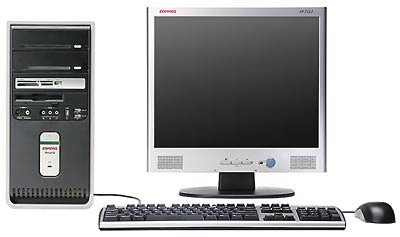
\includegraphics[width = 5cm]{img/s01/uc_ecran_clavier.png}
    \end{column}
  \end{columns}
  \vspace{1cm}
  \begin{columns}
    \begin{column}[l]{6cm}
      \begin{block}{Des formes très variées}
        \begin{itemize}
        \item Les ordinateurs modernes sont multiformes,
        \item Ils remplissent des tâches très variées.
        \end{itemize}
      \end{block}
    \end{column}
    \begin{column}[l]{5cm}
      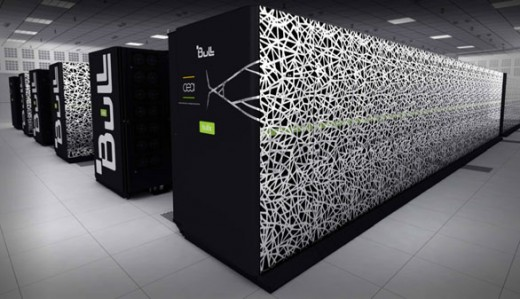
\includegraphics[width = 2.5cm]{img/s01/cluster_cea.png}\hspace{1cm}
      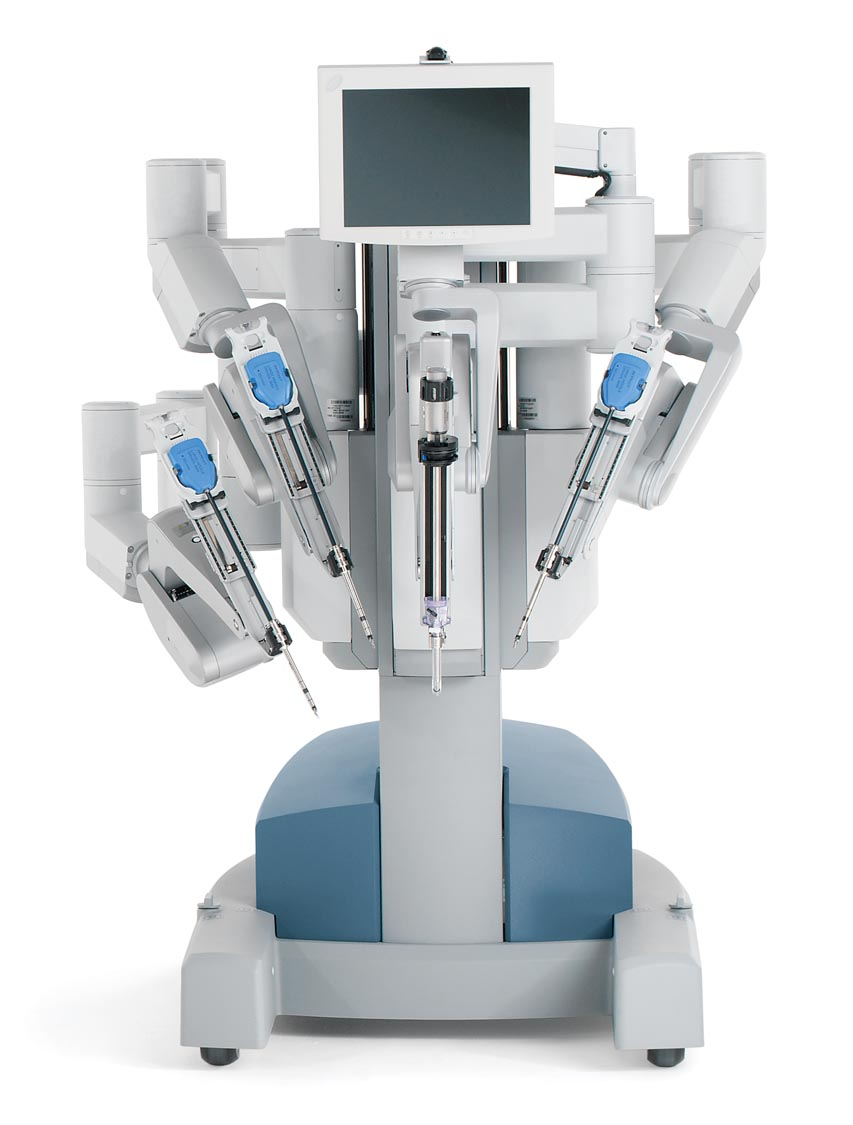
\includegraphics[height = 1.5cm]{img/s01/Davinci-Robot-chirurgical-001.jpg}\\
      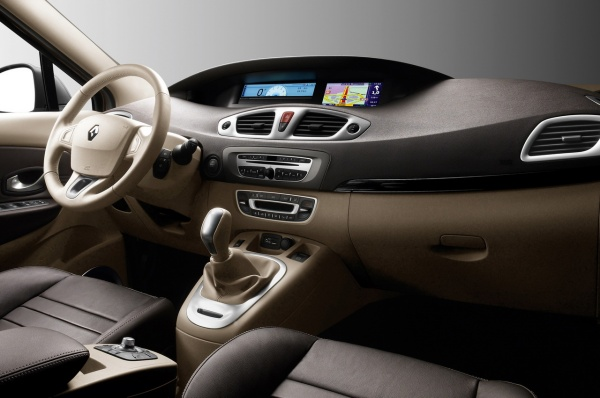
\includegraphics[width =
      2.5cm]{img/s01/scenic_console_centrale.png}\hspace{1cm}
      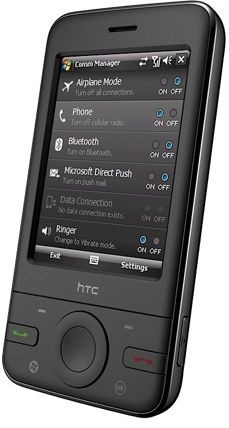
\includegraphics[height = 1.5cm]{img/s01/telephone_tc_linux.png}
    \end{column}
  \end{columns}
\end{frame}

\begin{frame}{Points communs et différences}
  \begin{block}{Matériel commun}
    \begin{itemize}
    \item Des capacités de calcul: CPU et/ou GPU
    \item De la mémoire : RAM, Disque dur, \dots
    \end{itemize}
  \end{block}
  \begin{block}{Logiciels similaires}
    \begin{itemize}
    \item Pour dialoguer avec le matériel : Système d'exploitation, Firmware
    \item Pour accomplir ses tâches : logiciels, programmes, \dots
    \end{itemize}
  \end{block}
  \begin{alertblock}{Périphériques différents}
    \begin{itemize}
    \item Interfaces : Connexions réseau, écrans, claviers, \dots
    \end{itemize}
  \end{alertblock}
\end{frame}
\begin{frame}{La carte mère}
  \centerline{%
    \only<1|handout:0>{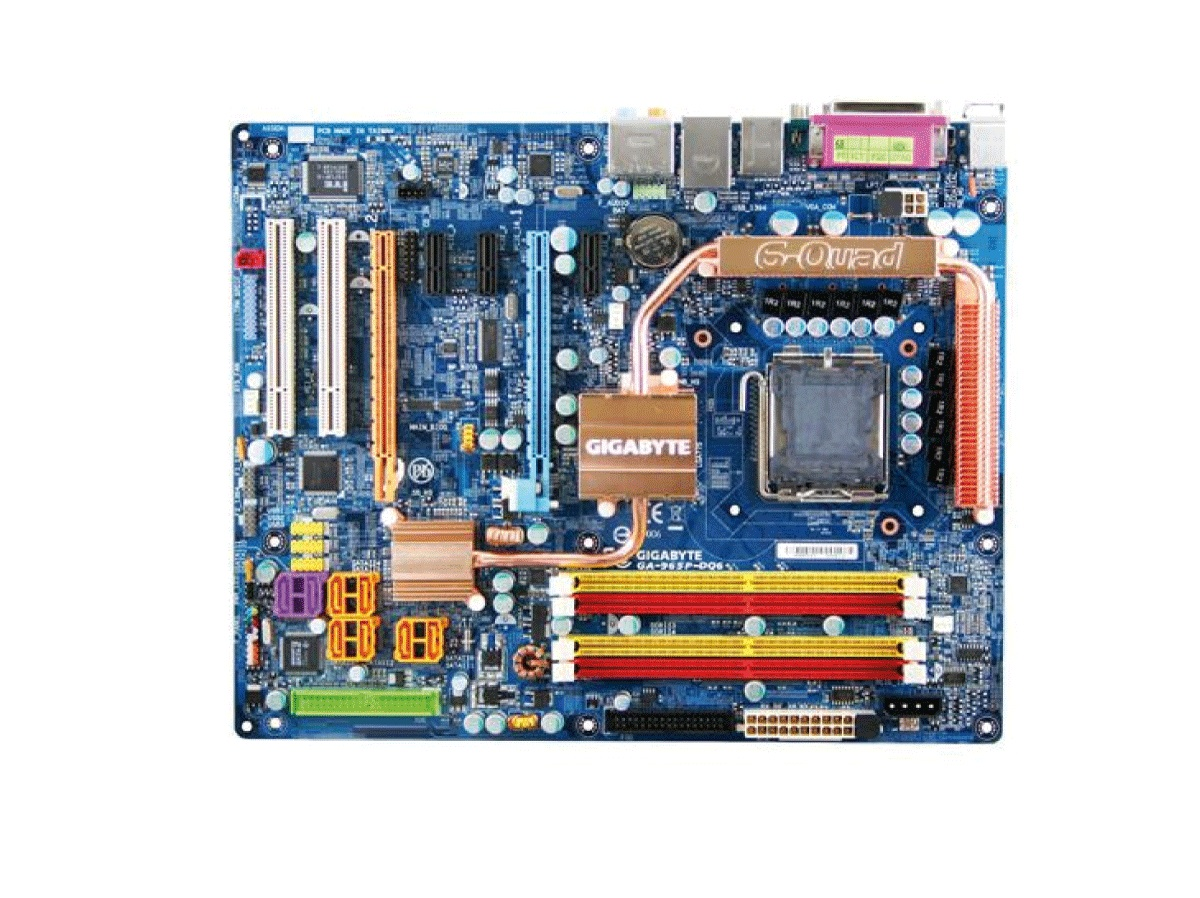
\includegraphics[width=.75\linewidth]{img/s01/carte_mere_commentee_1.jpg}}%
    \only<2|handout:1>{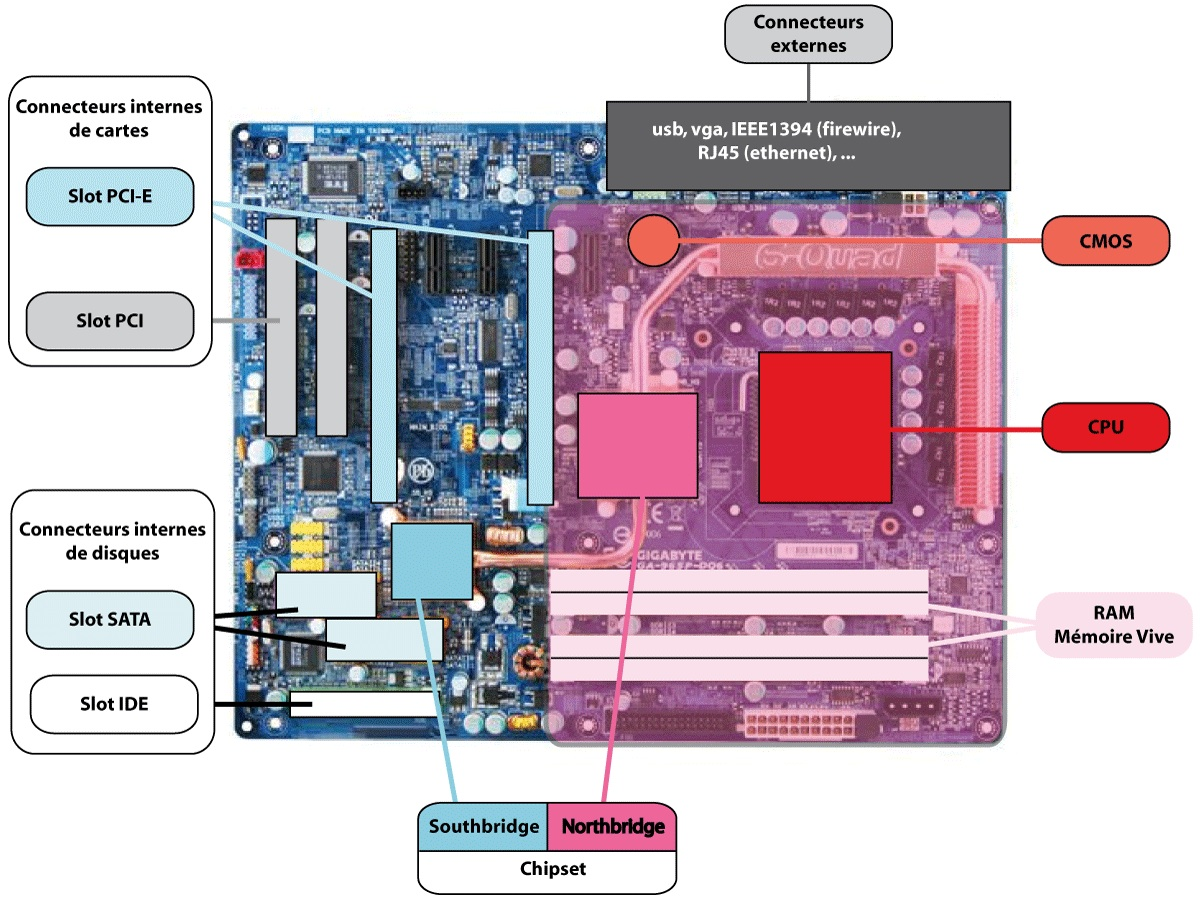
\includegraphics[width=.75\linewidth]{img/s01/carte_mere_commentee_2.jpg}}%
  }

  La carte mère est l'élément central de l'ordinateur sur lequel sont
  assemblés et mis en relation tous les composants matériels. Elle
  permet à tous ses composants de fonctionner ensemble efficacement.
\end{frame}

\begin{frame}{Les unités de calcul}
  \center 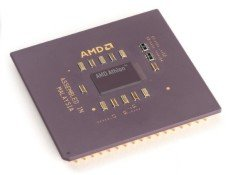
\includegraphics[height = 3 cm]{img/s01/CPU.png}
  \begin{block}{CPU - Central Processing Unit}
    \begin{itemize}
    \item C'est une puce qui traite des instructions élémentaires en
      réalisant des calculs binaires,
    \item Fréquence de l'ordre de 3 GHz.
    \end{itemize}
  \end{block}
  \begin{block}{GPU - Graphics Processing Unit}
    C'est une puce placée sur les cartes graphiques
    \begin{itemize}
    \item Elle prend en charge les nombreux calculs de rafraichissement
      des images 3D
    \item Une carte graphique moderne peut compter une grande quantité
      de ces puces.
    \end{itemize}
  \end{block}
\end{frame}

\begin{frame}{Des mémoires différentes pour des usages différents}
  \begin{columns}
    \only<1|handout:1>{
      \begin{column}{.65\linewidth}
        \begin{block}{ROM : Read Only Memory}
          \begin{itemize}
          \item Mémoire non-volatile maintenue par une conception
            physique,
          \item Taille limitée car très chère, très rapide,
          \item Contient instructions d'amorçage, routines\dots
          \end{itemize}
        \end{block}
        \begin{block}{RAM : Random Access Memory}
          \begin{itemize}
          \item Mémoire volatile: maintenue par une tension électrique,
          \item Accès rapide,
          \item Taille limitée car assez chère.
          \end{itemize}
        \end{block}
        \begin{block}{Disque Dur, clef-usb, \dots}
          \begin{itemize}
          \item Mémoire non-volatile (enregistrement magnétique le plus
            souvent),
          \item Accès lent,
          \item Taille très grande (support de stockage de masse),
            beaucoup moins chère.
          \end{itemize}
        \end{block}
      \end{column}
    } \only<2|handout:2>{ 
      \begin{column}{.65\linewidth}
        \begin{block}{Organisation de la mémoire}
          Les ordinateurs réalisent des calculs logiques sur des données
          binaires\
          \begin{itemize}
          \item Les données et les instructions sont stockées sous forme
            de blocs repérés par une adresse,
          \item Les blocs contiennent une information binaire organisée
            en octet. Chaque octet contient 8 bits d'information qui
            sont lus comme une suite ordonnée de 0 ou de 1 ou de Vrai et
            de Faux.
          \item Un octet peut prendre $2^8=256$ valeurs différentes.
          \end{itemize}
        \end{block}
        \centerline{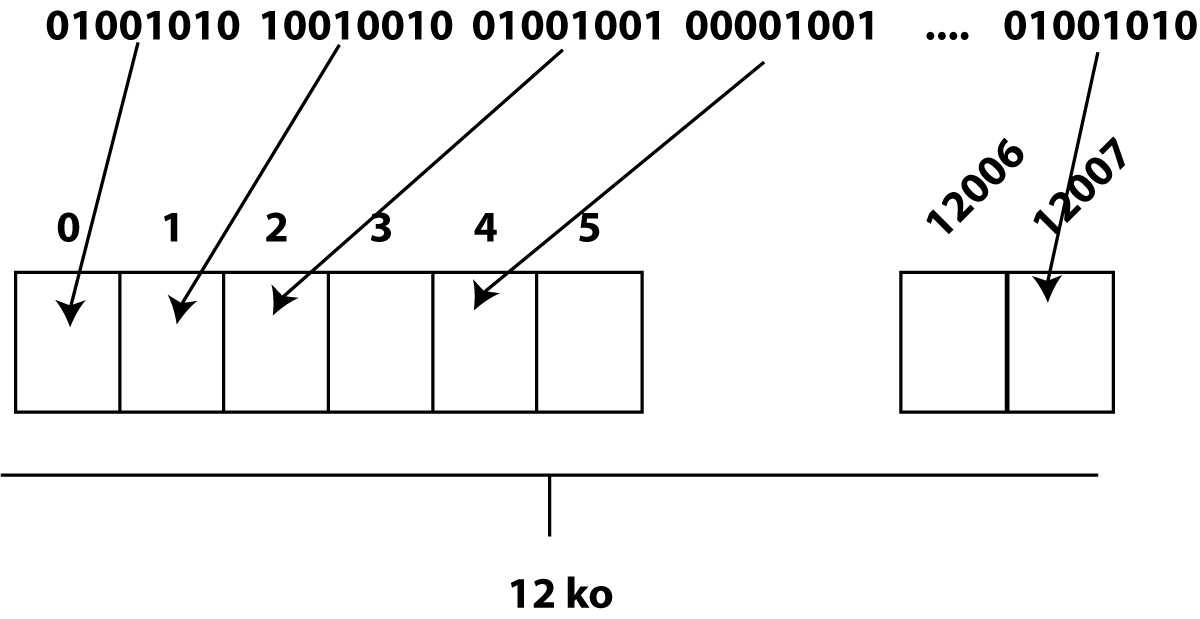
\includegraphics[height=3cm]{img/s01/Memoire.jpg}}
      \end{column}
    }%
    \begin{column}{.3\linewidth}
      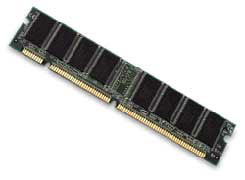
\includegraphics[width=\linewidth]{img/s01/RAM.png}\\
      \vspace{1cm}
      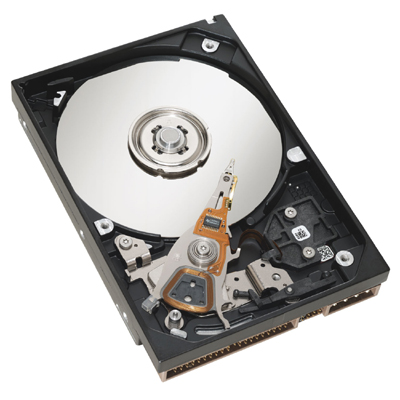
\includegraphics[width=\linewidth]{img/s01/disque_dur.png}
    \end{column}
  \end{columns}
\end{frame}
\begin{frame}{Les périphériques}
  \begin{block}{Des composants externes}
    En fonction de leur tâche, de nombreux composants \textit{ad hoc}
    peuvent être \textit{greffés} sur la structure de base précédemment
    décrite. Par exemple:
    \begin{itemize}
    \item Ordinateur de Maison: Écran, souris, imprimante, scanner,
      joystick, modem, \dots
    \item Ordinateurs de bord: Sondes, actioneurs, \dots
    \item Télephone: Antenne, récepteurs, \dots
    \item Robot médical: Interface haptique, bras mécaniques, \dots
    \end{itemize}
  \end{block}
  \begin{block}{Des composants internes}
    En fonction des possibilités des cartes mères plusieurs types de
    composants peuvent être ajoutés:
    \begin{itemize}
    \item Cartes vidéo, Cartes son, disques durs internes, lecteurs,
      \dots
    \item Cartes d'acquisition ou de pilotage de périphériques, \dots
    \end{itemize}
  \end{block}
  \begin{center}
    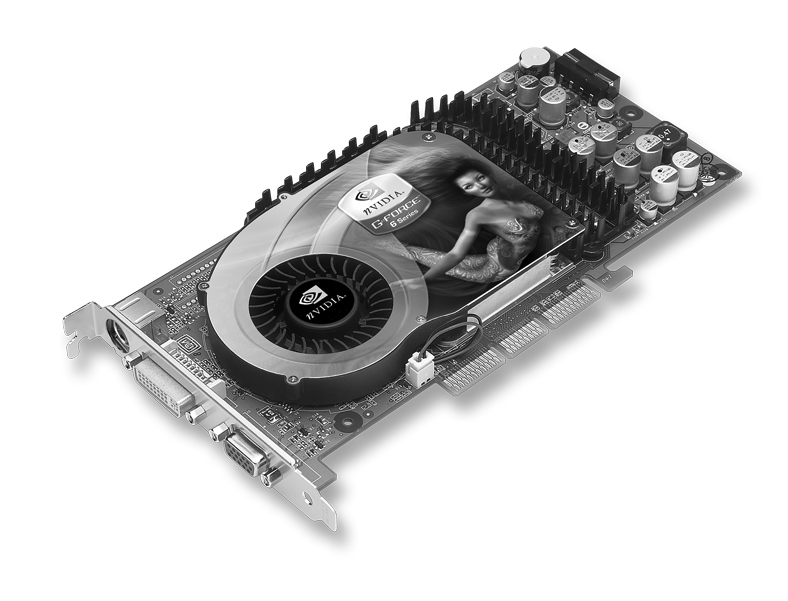
\includegraphics[height=2cm]{img/s01/carte_video.png}
    \hspace{2cm}
    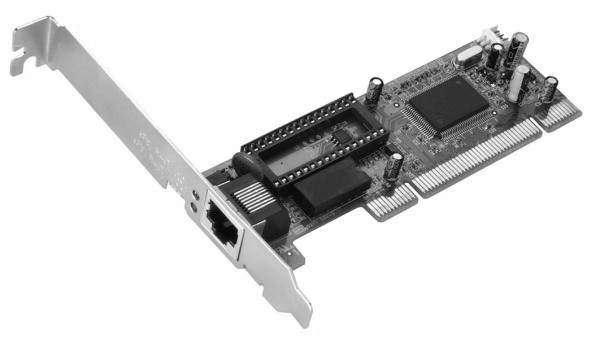
\includegraphics[height=2cm]{img/s01/carte_reseau.png}
  \end{center}
\end{frame}

\begin{frame}{Les bus}
  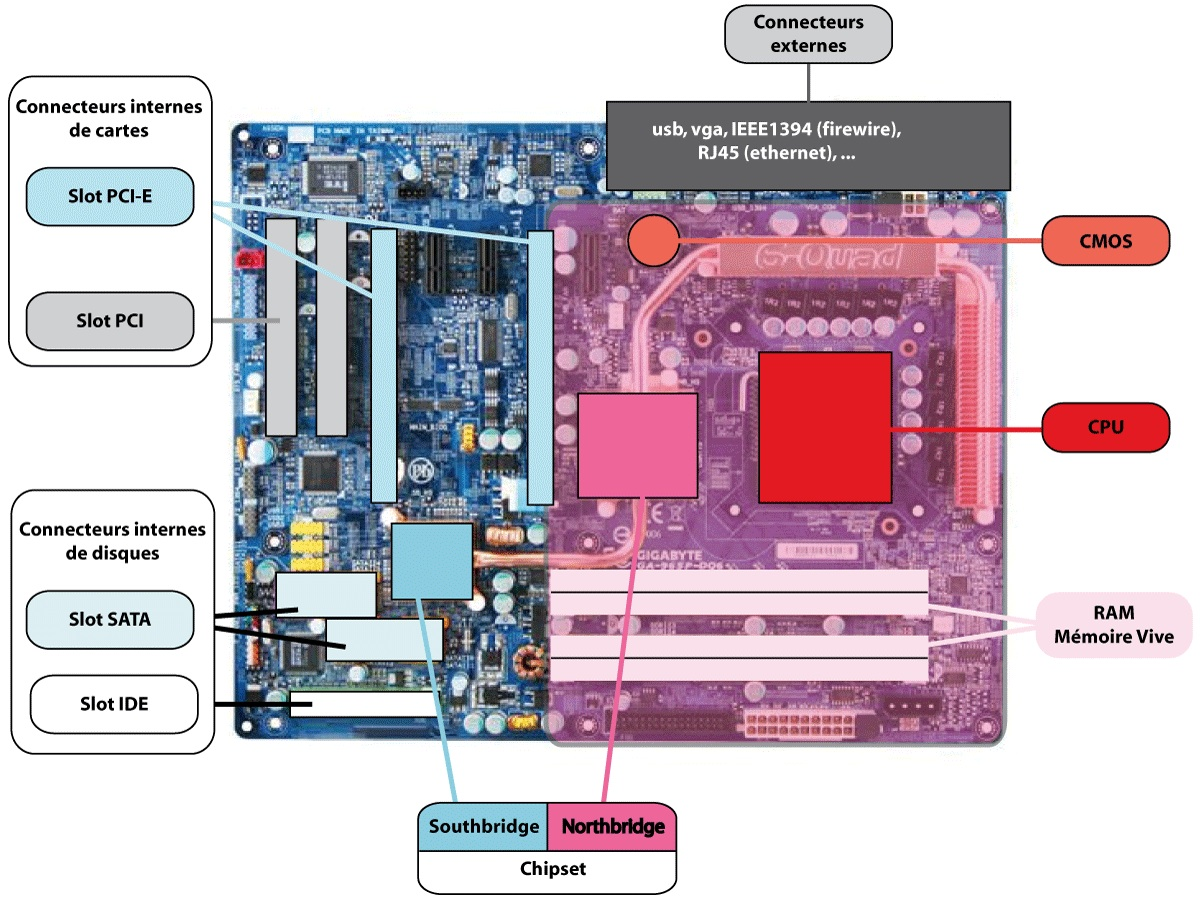
\includegraphics[width=6cm]{img/s01/carte_mere_commentee_2.jpg}%
  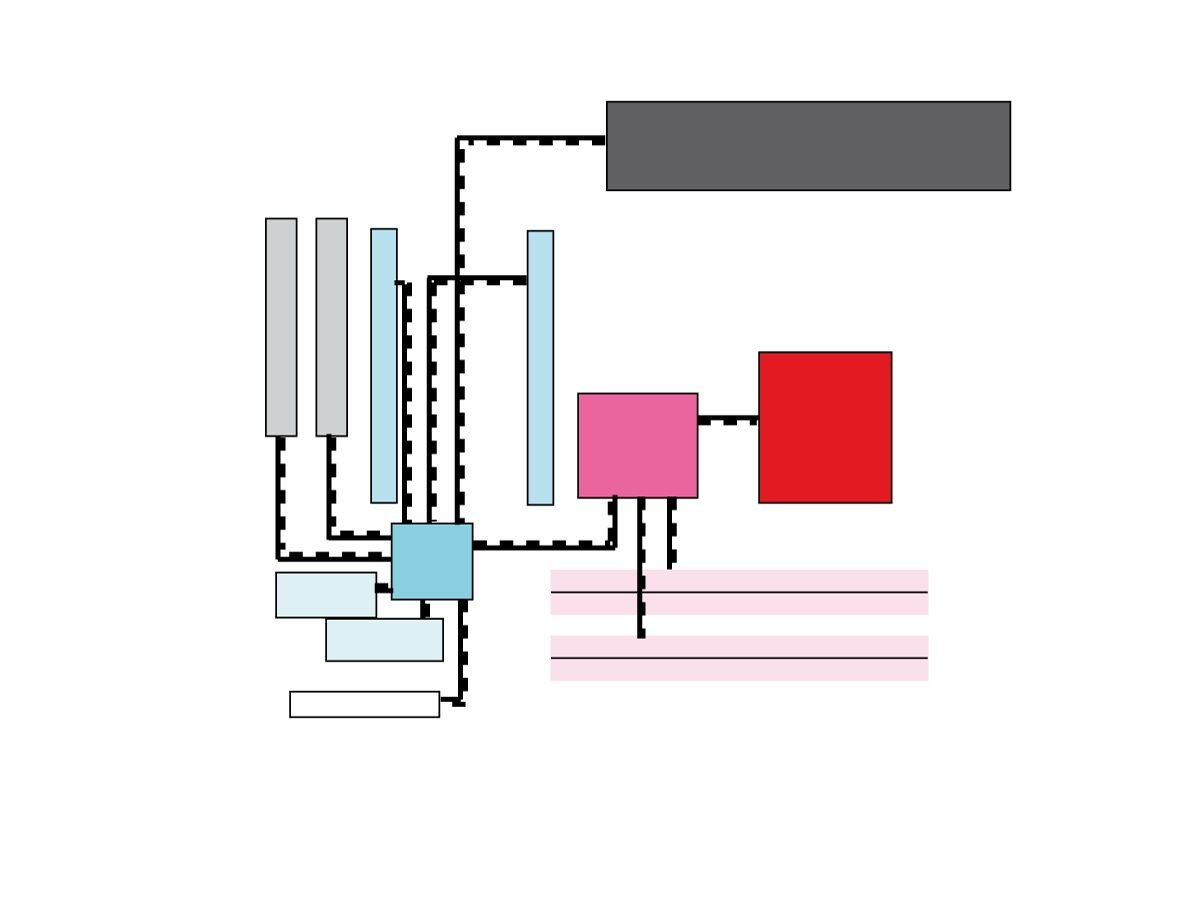
\includegraphics[width=6cm]{img/s01/carte_mere_commentee_3.jpg}%
  \begin{block}{La carte mère intègre les bus.}
    \begin{itemize}
    \item Les bus sont des unités physiques qui assurent le transport
      efficace de l'information entre les différents composants
      connectés à la carte mère,
    \item La largeur (8, 16, 32 64 bits), série ou parallèle et la
      fréquence ($10^2-10^3$ MHz) des bus règlent le débit d'information
      entre les composants. Cela conditionne donc fortement l'efficacité
      d'une configuration matérielle.
    \end{itemize}
  \end{block}
\end{frame}

\begin{frame}{Conclusion:~L'horizon matériel}
  \begin{block}{Interaction avec le matériel}
    \begin{itemize}
    \item Heureusement le programmeur ou l'utilisateur n'interagit pas
      directement avec le matériel (sauf pour remplacer une pièce
      défectueuse ou connecter un nouveau matériel \dots). Le dialogue
      avec l'architecture matériel est l'affaire de programmes dédiés.
    \item Plusieurs couches logicielles existent entre le matériel et
      l'utilisateur: les \textit{firmwares}, le noyau du système et les
      outils et programmes du système d'exploitation.
    \item La plupart des logiciels que vous serez amené à développer
      n'interagiront qu'indirectement avec le matériel par le filtre des
      librairies système.
    \end{itemize}
  \end{block}
  \begin{alertblock}{Haut Niveau $\rightarrow$}
    \begin{itemize}
    \item Logiciel,langages de programmation, \dots
    \item[\dialoginformation] C'est le domaine de l'informatique et des informaticiens
    \item[\dialogsystem] Une interface: Le système d'exploitation
    \end{itemize}
  \end{alertblock}
  \begin{alertblock}{Bas niveau}
    \begin{itemize}
    \item \textit{Firmwares}, exécution des instructions machine,
      \dots
    \item C'est le domaine de la physique et des électroniciens.
    \end{itemize}
  \end{alertblock}
\end{frame}

\section{Le système d'exploitation}
\label{sec:OSGeneralites}
\subsection{La fonction du système d'exploitation}
\begin{frame}{Le système d'exploitation}
  Le système d'exploitation permet de développer des programmes sans
  tenir compte de la complexité physique de la machine. Les programmes
  utilisent des fonctionnalités standardisées d'accès aux ressources
  matérielles.
  \begin{columns}
    \begin{column}{5.5cm}
      \begin{block}{Côté Système, l'O.S.}
        \begin{itemize}
        \item coordonne l'utilisation des ressources (par exemple temps CPU
          accordé à chaque processus, allocation mémoire, \dots),
        \item assure la maintenance et la fiabilité du système (par exemple
          gestion des fichiers, de la sécurité informatique, \dots)
        \item \dots
        \end{itemize}
      \end{block}
      \begin{block}{Côté utilisateur, l'O.S.}
        \begin{itemize}
        \item facilite l'accès et l'utilisation des ressources
          matérielles,
        \item propose une interface de programmation permettant
          d'utiliser ces matériels
        \item \dots
        \end{itemize}
      \end{block}
    \end{column}
    \begin{column}{6cm}
      \begin{center}
        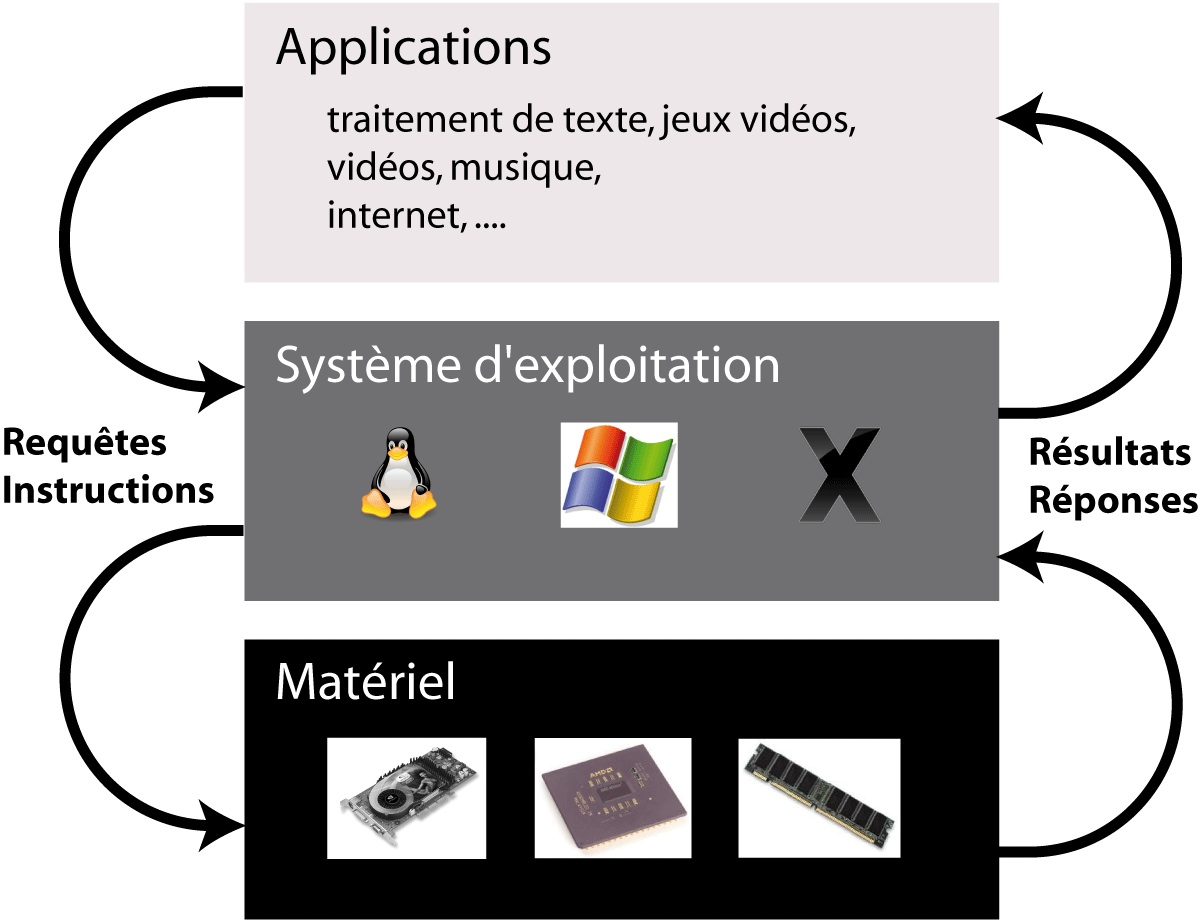
\includegraphics[width=6cm]{img/s01/OS_interface_2.jpg}
      \end{center}
    \end{column}
  \end{columns}
\end{frame}

\subsection{La multiplicité des systèmes existants}
\begin{frame}{Les différents systèmes d'exploitation}
  \begin{columns}
    \begin{column}{5.5cm}
      \begin{block}{Beaucoup d'OS différents existent:}
        Chaque architecture matérielle  demande un système d'exploitation adapté. Certain systèmes d'exploitation sont plus souples et prennent en charge des architectures matérielles multiples.
      \end{block}
      \begin{center}
        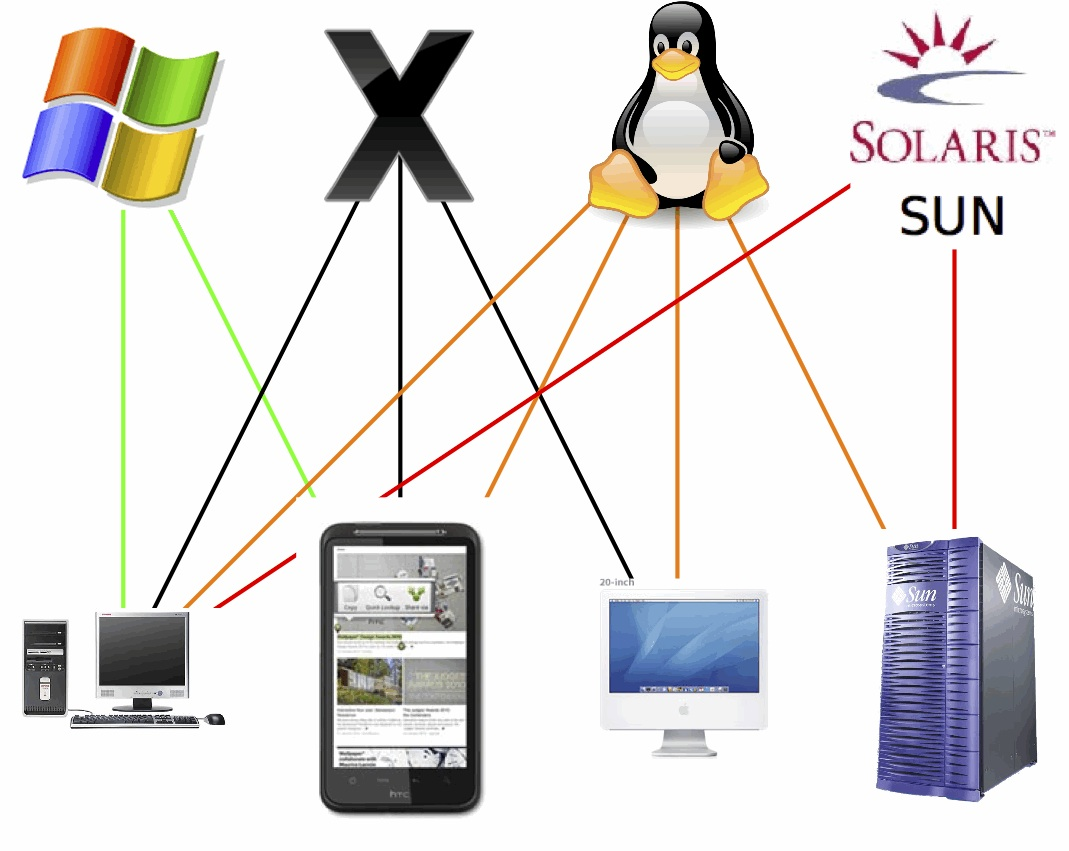
\includegraphics[width=5.5cm]{img/s01/OS_archi.jpg}
      \end{center}
    \end{column}
    \begin{column}{5.5cm}
      \begin{block}{Deux OS se distinguent:}
        Windows est le système d'exploitation le plus utilisé, et Linux est le système d'exploitation le plus souple.\\
        Statistiques au 5 janvier 2011: \url{http://gs.statcounter.com/}\\
        \begin{itemize}
        \item 95\% des ordinateurs utilisent Windows,
        \item il existe plus de 600 Systèmes Linux\dots
        \end{itemize}
      \end{block}
      \vrule
      \begin{center}
        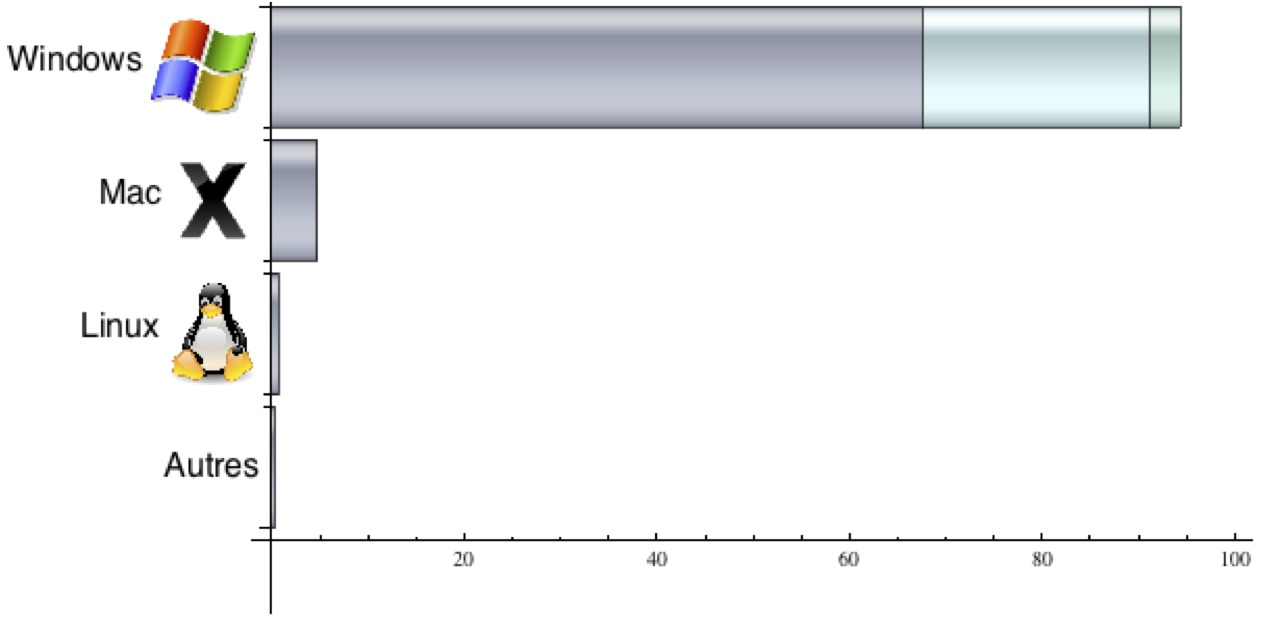
\includegraphics[width=5.5cm]{img/s01/OS_utilises.jpg}
      \end{center}
    \end{column}
  \end{columns}
\end{frame}

\subsection{Comparatif}
\begin{frame}{Les différents systèmes d'exploitation}
  \begin{columns}
    \begin{column}{58mm}
      \begin{block}{\center 
\includegraphics[height=1cm]{img/s01/Tux.png}\\Linux}
        \begin{itemize}
        \item Non propriétaire: Gratuit le plus souvent
        \item Ouvert: sources disponibles
        \item Flexible: sources modifiables
        \item Puissant: Programmable
        \item Communauté active: entraide des utilisateurs
        \item Plus complexe: plutôt pour les informaticiens (interfaces
          de programmation optimisées)
        \end{itemize}
      \end{block}
    \end{column}
    \begin{column}{58mm}
      \begin{block}{\center 
\includegraphics[height=1cm]{img/s01/Windows_logo.png}\\Windows}
        \begin{itemize}
        \item Propriétaire: Payant
        \item Sources non disponibles
        \item Sources non modifiables
          % \item Plus difficilement programmable
        \item Communauté active: nombreux utilisateurs
        \item Plus ergonomique: pour les utilisateurs (interfaces
          d'utilisation optimisées)
        \end{itemize}
        \vrule
      \end{block}
    \end{column}
  \end{columns}
  \begin{alertblock}{Linux un système puissant en constante évolution}
    Depuis une dizaine d'année, Linux a beaucoup évolué. La plupart des
    distributions proposent des systèmes d'installation automatisés, des
    outils de bureautique ressemblant aux suites commerciales. Il
    bénéficie en outre d'une sécurité accrue à l'heure des virus et
    autres failles de sécurité.
  \end{alertblock}
\end{frame}

\section{Le système Linux}
\subsection{Un peu d'histoire}
\begin{frame}{Un peu d'histoire}
  \begin{block}{GNU-Linux}
    \begin{itemize}
    \item Le système GNU-Linux est la rencontre d'une technologie, le
      noyau Linux et d'une philosophie de développement et de
      diffusion. C'est un système au développement collaboratif (par une
      communauté) qui est distribué librement et permet l'utilisation de
      tous les logiciels libres développés pour son architecture.
    \item Le noyau Linux est historiquement une version libre du système
      UNIX développé initialement par le Finlandais Linus Torvalds à
      partir du début des années 1990.
    \item Le projet GNU est celui du développement collaboratif et libre
      d'un système d'exploitation libre initié par Richard Stallman en
      1983.
    \end{itemize}
  \end{block}
  \begin{block}{Ahjourd'hui}
    \begin{itemize}
    \item C'est un système très largement diffusé et utilisé sur lequel
      ont été développées plusieurs distributions (qui sont des suites
      logicielles qui accompagnent le noyau).
    \item Initialement confidentiel et réservé à des spécialistes avec
      des interfaces rudimentaires, il est aujourd'hui toujours plus
      ergonomique et automatisé pour les non spécialistes, mais laisse
      les outils et interfaces de bas niveau disponibles au plus grand
      nombre.
    \item On notera par exemple l'existence de nombreuses interfaces
      graphiques \textit{Bureaux} (GNOME, KDE, \dots) de nombreux
      paquetages pré-compilées, de nombreux outils d'administration et
      de services (protocoles, \dots)
    \end{itemize}
  \end{block}
  
\end{frame}
\subsection{Gentoo: La distribution utilisée à l'IUT}
\begin{frame}{À l'IUT: Gentoo}
  \begin{block}{Une distribution téléchargeable}
    \begin{columns}
      \begin{column}{8cm}
        \url{http://www.gentoo.org/}\\
        \url{http://fr.gentoo-wiki.com/wiki/Accueil}
      \end{column}
      \begin{column}{3cm}
        
\includegraphics[width=1cm]{img/s01/gentoo_logo.png}
      \end{column}
    \end{columns}
  \end{block}
  \begin{block}{Pour ce cours}
    \begin{itemize}
    \item Les concepts abordés dans ce module sont généraux.
    \item Il pourront être testés sur tous les systèmes Linux (avec de très faibles variantes).
    \item Il vous est possible d'installer une version de Linux sur votre ordinateur personnel (installation ou version Live) pour votre pratique personnelle et la préparation de l'examen.
    \item Une pratique régulière devrait vous assurer une bonne note à peu de frais\dots
    \end{itemize}
  \end{block}
  \begin{alertblock}{Pour vous préparer à l'examen}
    Il vous est possible:
    \begin{itemize}
    \item d'utiliser Linux dans les salles machines,
    \item d'utiliser Linux via le service de bureaux virtuels \textit{via} le portail de l'université:\\ \url{https://portail.cevif.univ-paris13.fr/}
    \item d'installer une version de Linux sur votre ordinateur personnel (installation ou version Live).
    \end{itemize}
  \end{alertblock}
\end{frame}

\subsection{Un système multi-utilisateurs}
\begin{frame}{Un système Multi-Utilisateurs}
  \begin{block}{Des utilisateurs et des droits}
    \begin{itemize}
    \item Chaque personne accédant au système est identifiée par un
      \textbf{nom d'utilisateur} (dit \textit{login}) et un mot de passe
      (dit \textit{password}).
    \item Chaque utilisateur bénéficie de permissions: exécution de
      certains programmes, lecture de certaines données, écriture de
      fichiers dans une limite de taille et dans seulement certains
      répertoires.
    \item Chaque utilisateur bénéficie d'un espace de travail réservé
      sur le disque. Cet espace de travail est un répertoire de
      l'arborescence dans lequel l'utilisateur à tous les droits: il
      peut y créer des sous-répertoires, y écrire des fichiers, y
      installer des programmes et applications. Toutes ses données et
      préférences personnelles y sont regroupées.
    \item Ce répertoire est appelé "Répertoire Personnel" ou
      \textit{"Home Directory"}. Il est en général placé dans un
      répertoire qui s'appelle \lin{/home/} et porte le nom de
      l'utilisateur : \lin{/home/nom\_utilisateur/}.
    \end{itemize}
  \end{block}
  \begin{alertblock}{Superutilisateur - Root}
    \begin{itemize}
    \item certains utilisateurs ont des permissions étendues pour
      administrer le système et effectuer des opérations interdites à
      l'utilisateur normal.
    \item l'utilisateur \lin{root} a tous les droits dans le système
      (par exemple il peut changer les permissions de n'importe quel
      fichier, il fixe les noms d'utilisateur et les mots de passe, il
      peut installer des programmes et librairies dans les répertoires
      système, \dots)
    \end{itemize}
  \end{alertblock}
\end{frame}

\begin{frame}{Identification en 2 étapes}
  \begin{center}
    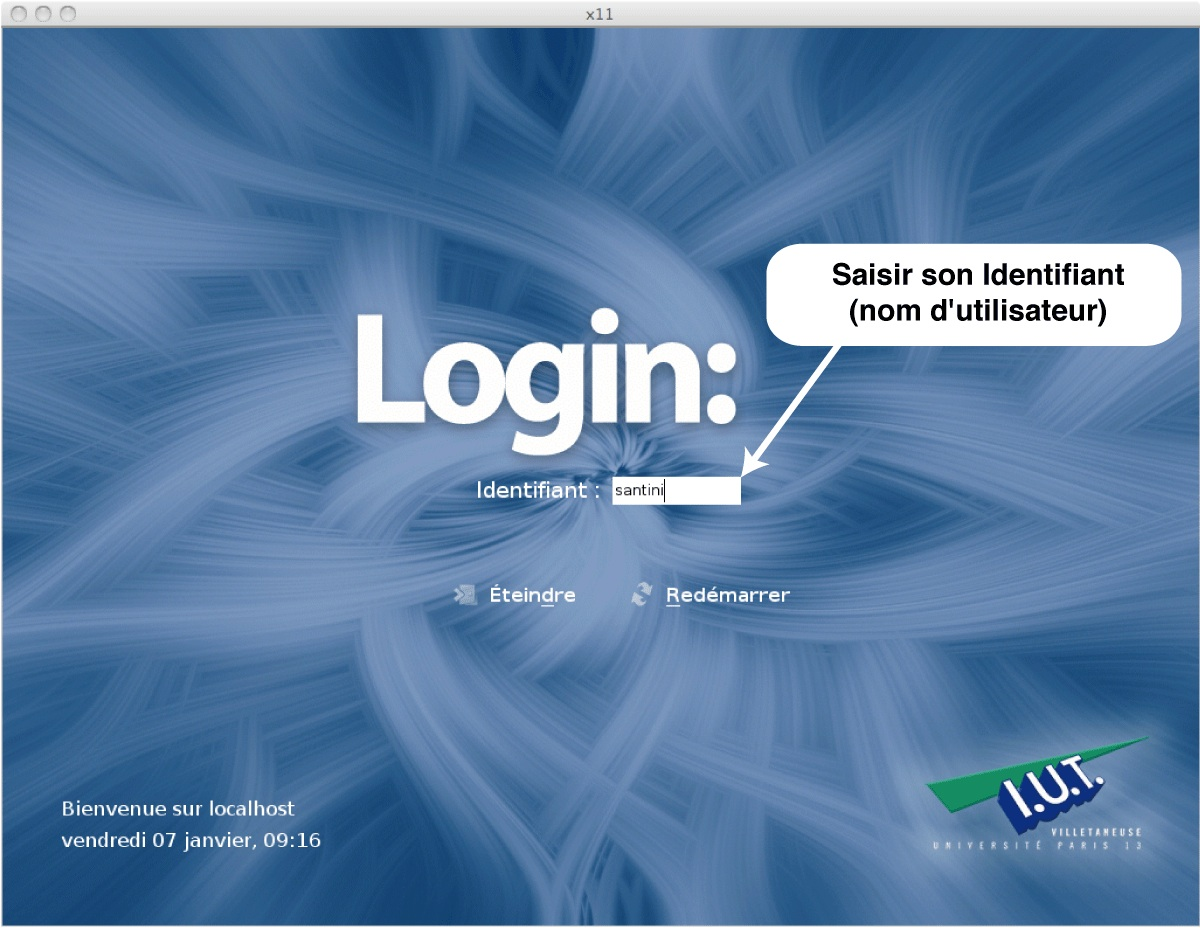
\includegraphics[width=8cm]{img/s01/linux_login.jpg}
  \end{center}
  \begin{block}{Étape \#1}
    S'identifier en donnant au système son nom d'utilisateur
  \end{block}
\end{frame}
\begin{frame}{Identification en 2 étapes}
  \begin{center}
    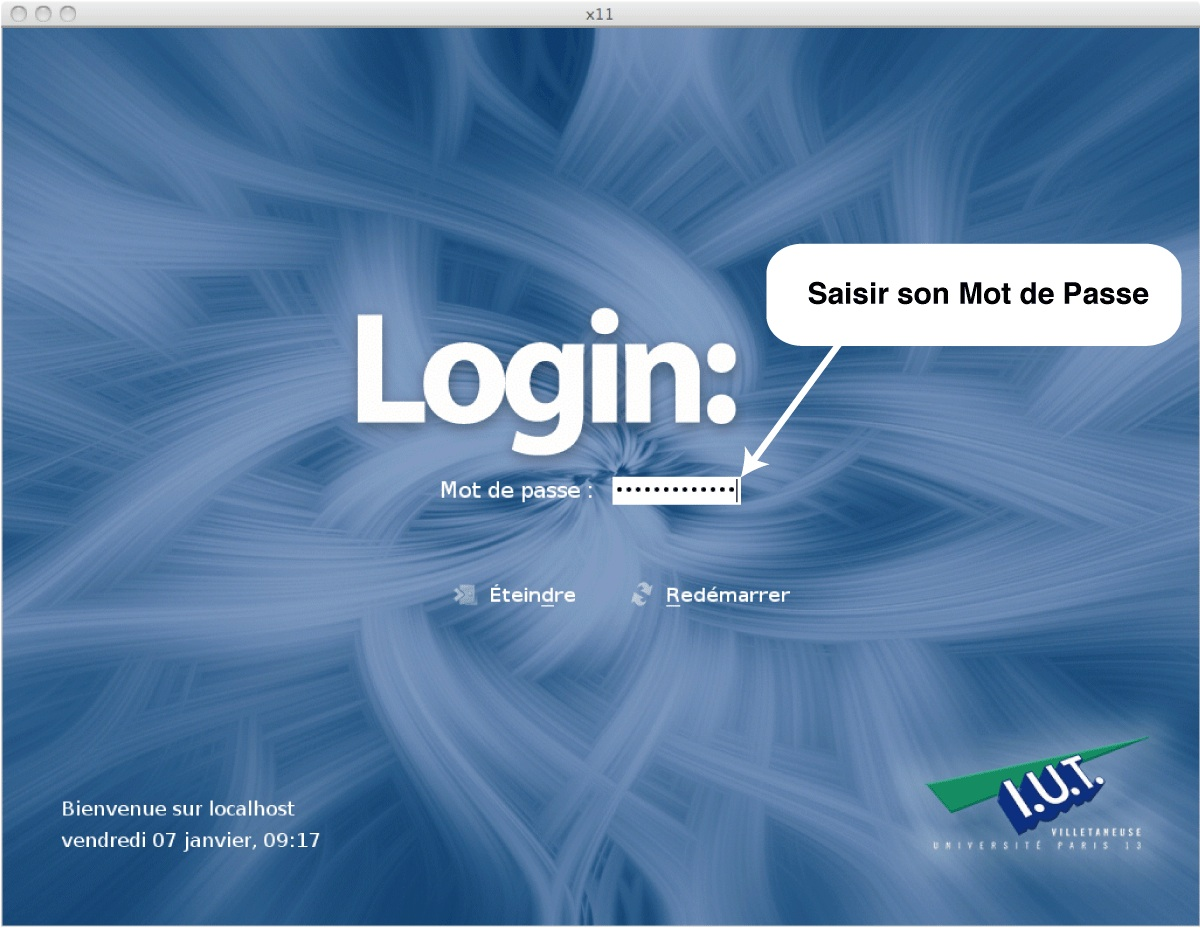
\includegraphics[width=8cm]{img/s01/linux_passwd.jpg}
  \end{center}
  \begin{block}{Étape \#2}
    Valider son identité avec le mot de passe
  \end{block}
\end{frame}

\subsection{Une interface graphique}
\begin{frame}{Accès au système}
  \begin{center}
    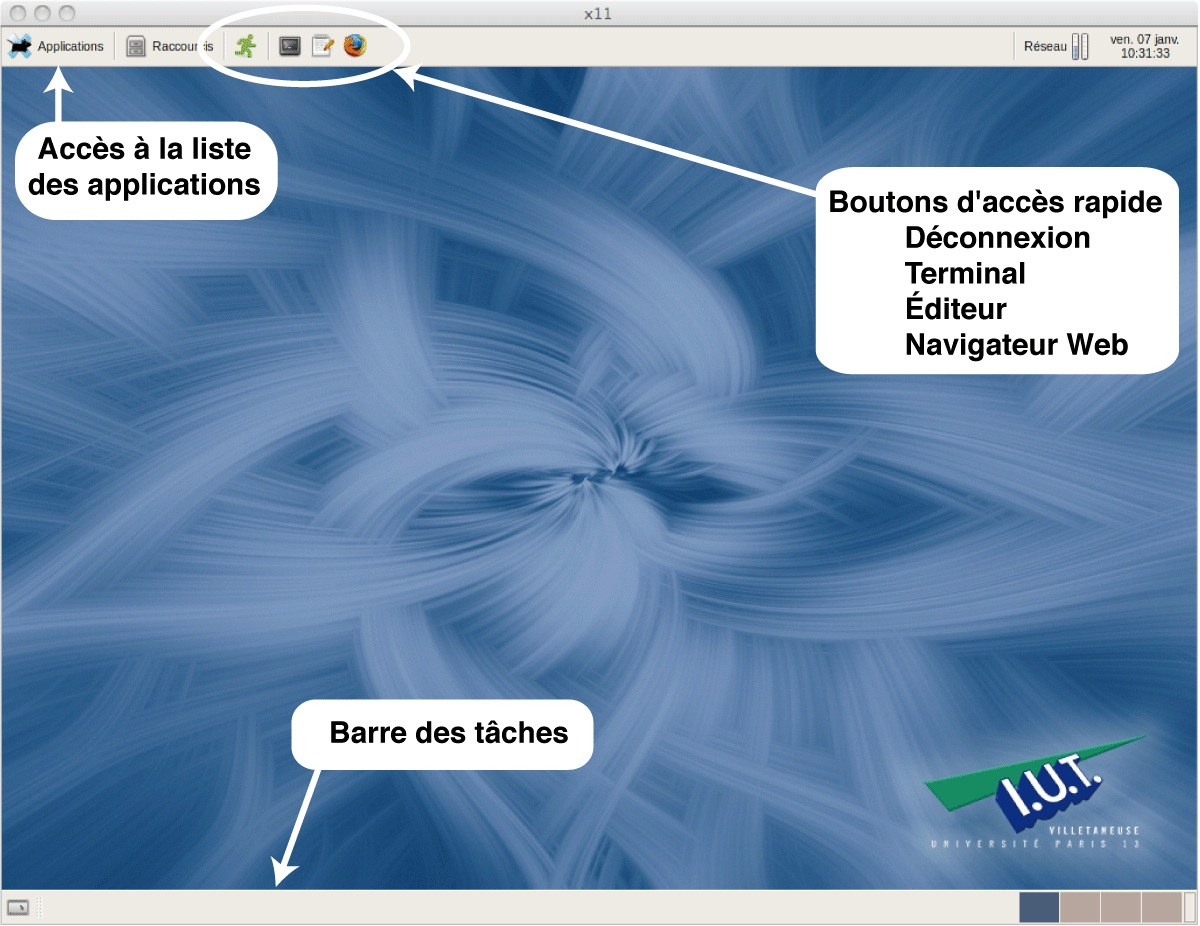
\includegraphics[width=8cm]{img/s01/Gnome_desktop.jpg}
  \end{center}
  \begin{block}{Le bureau GNOME}
    Parmi les différents environnements graphiques existants, vous
    utiliserez l'environnement GNOME (\url{http://www.gnomefr.org/}).
  \end{block}
\end{frame}

\subsection{Les logiciels disponibles}
\begin{frame}{Les logiciels disponibles}
  \begin{block}{Les suites bureautiques}
    \begin{itemize}
    \item Les suites bureautiques proposent les fonctionnalités grand
      public de traitement de texte, de tableur, de présentation, de
      dessin.
    \item Plusieurs suites gratuites existent en libre accès sous linux
      \begin{itemize}
      \item CalligraSuite (\url{http://www.calligra-suite.org/})
      \item OpenOffice (\url{http://fr.openoffice.org/})
      \item \dots
      \end{itemize}
    \end{itemize}
  \end{block}
  \begin{block}{Les programes dédiés}
    \begin{itemize}
    \item Navigateur Web, Client de messagerie, comme sous d'autres OS,
      de nombreuses solutions existent.
      \begin{itemize}
      \item Firefox, Opera, Konqueror, \dots
      \item Thunderbird, KMail, \dots
      \end{itemize}
    \item Des logiciels parmi les plus puissants:
      \begin{itemize}
      \item Manipulation et création d'images: GIMP, ImageMagick, \dots
      \item Modélisation 3D: Blender, \dots
      \end{itemize}
    \end{itemize}
  \end{block}
  \begin{block}{De nombreuses micro-application ou programmes}
    \begin{itemize}
    \item De nombreux programmes de conversion de format, de
      communication et de téléchargement existent en ligne de commande
      \dots
    \end{itemize}
  \end{block}
\end{frame}

\subsection{Distribution et accès aux logiciels}
\begin{frame}{Distribution et accès aux logiciels}
  \begin{columns}
    \begin{column}{6cm}
      \begin{block}{Licences libres (open source)}
        Elles permettent de :
        \begin{itemize}
        \item d'utiliser le logiciel,
        \item d'étudier et de modifier les sources,
        \item de redistribuer les sources, modifiées ou non.
        \end{itemize}
      \end{block}
    \end{column}
    \begin{column}{5cm}
      \begin{block}{Licences Propriétaires}
        Elles restreignent un ou plusieurs des droits listés \it{supra}.
      \end{block}
      \begin{block}{Gratuit ne signifie pas libre}
        Certains logiciels gratuits sont des logiciels propriétaires).
      \end{block}
    \end{column}
  \end{columns}
  \begin{block}{Copyright\copyright{} vs Copyleft\textcopyleft}
    Elles permettent de : Distribué en Copyleft\textcopyleft, les
    sources modifiées préservent les droits précédents.  $\Rightarrow$
    Les logiciels qui dérivent des sources Copyleft ne peuvent être
    distribués avec un Copyright\copyright.
  \end{block}
  \begin{block}{Tout logiciel a un coût de développement}
    En général:
    \begin{itemize}
    \item Propriétaire est payant: On paie un coût de développement, un
      service de support, un service de mise à jour, ... Les sources
      sont protégées et seuls les propriétaires y ont accès.
    \item Libre est gratuit: Le coût est supporté par une communauté
      (utilisateurs, subventions publiques, subventions ou sociétés
      privées, \dots).
    \end{itemize}
  \end{block}
\end{frame}
\endinput


\subsection{La ligne de commande}
\begin{frame}{La ligne de commande}
  \begin{block}{Interface de communication avec le système (IHM)}
    \begin{itemize}
    \item Interface historique en mode texte,
    \item Interface privilégiée sous Linux: de nombreux programmes ne peuvent être appelés qu'à partir de la ligne de commande,
    \item Interface puissante et programmable. 
    \end{itemize}
  \end{block}
  \begin{block}{Principes de fonctionnement}
    \begin{enumerate}
    \item L'utilisateur tape des commandes sous forme de texte
    \item Le texte est évalué par un interpréteur,
    \item L'interpréteur lance l'exécution des commandes.
    \end{enumerate}
  \end{block}
  \begin{block}{Utilité}
    \begin{itemize}
    \item Permet de lancer des programmes ou des applications,
    \item Permet d'interroger le système et d'interagir avec lui.
    \item Basé sur un interpréteur, un langage de programmation permet de construire des scripts pour effectuer des tâches complexes de gestion ou d'administration.
    \end{itemize}
  \end{block}
\end{frame}
%%%%%%%%%%%%%% 
\begin{frame}{La ligne de commande}
  \begin{center}
    \mprompt{
      \prompt{\cursor}{}
    }
  \end{center}
  \begin{block}{La fenêtre de terminal ou Shell}
    La ligne de commande est un programme fenêtré simple qui permet de taper du texte.
    \begin{itemize}
    \item La ligne de commande comporte une partie non interprétée \lin{[ {\color{red} user}@{\color{ForestGreen} localhost} {\color{MediumBlue}\~{} }]} appelée le \textit{prompt}. Ici le prompt est configuré pour afficher le {\color{red}nom de l'utilisateur}, le {\color{ForestGreen}nom de la machine}, et le {\color{MediumBlue}nom du répertoire courant}.
    \item Le caractère \lin{\cursor} symbolise la position du curseur. C'est la position où sera inséré le texte frappé par l'utilisateur.
    \item Le texte tapé par l'utilisateur sera évalué comme une commande ou une suite de commandes par un interpréteur.
    \end{itemize}
  \end{block}
  \begin{block}{L'interpréteur}
    \begin{itemize}
    \item L'interpréteur parcourt le texte tapé par l'utilisateur, identifie les commandes et les paramètres, et si la syntaxe est correcte, lance un processus.
    \item Plusieurs interpréteurs existent: csh, tcsh, bash. Dans ce cours nous utiliserons le \textbf{bash}. 
    \item Bash acronyme de Bourne-Again shell, est l'interpréteur du projet GNU. Il est le plus utilisé sous linux.
    \end{itemize}
  \end{block}
\end{frame}
%%%%%%%%%%%%%% 
\begin{frame}{La ligne de commande}
  \begin{center}
    \mprompt{
      \prompt{ls}{public\_html/}\\
      \prompt{\cursor}{}
    }
  \end{center}
  \begin{block}{Exécution d'une commande}
    \begin{itemize}
    \item La commande (ici \lin{ls}) est évaluée (lancée, interprétée) dès que l'utilisateur presse la touche \Return (Entrée). L'ensemble du texte partant du prompt jusqu'à la fin de la ligne est interprété comme une commande.
    \item Si la commande est valide, un programme est lancé.
    \item Durant l'exécution du programme, la ligne de commande est indisponible. L'utilisateur doit attendre la fin de l'exécution du programme avant de pouvoir taper une nouvelle commande.
    \item Si le programme produit un affichage (ici \lin{ls} affiche le nom des fichiers et répertoires), celui-ci est affiché par défaut dans la fenêtre du Shell.
    \item Une fois la commande exécutée, le Shell propose une nouvelle ligne de commande où l'utilisateur peut taper une nouvelle instruction.
    \end{itemize}
  \end{block}
\end{frame}
%%%%%%%%%%%%%% 
\begin{frame}{La ligne de commande}
  \begin{center}
    \mprompt{
      \prompt{nom\_commande \textit{options paramètres}}{affichage\\\dots}\\
      \prompt{\cursor}{}
    }
  \end{center}
  \begin{block}{Interpretation de la commande}
    \begin{description}
    \item[nom\_commande] Le premier mot doit correspondre au nom d'une commande connue du système,
    \item[options] Comme le nom l'indique les options ne sont pas obligatoires. Si il n'y en a pas la commande s'exécute selon un mode "par défaut". L'ajout d'une option pourra modifier ce comportement par défaut.
    \item[paramètres] Certaines commandes peuvent fonctionner sans paramètre.
    \end{description}
  \end{block}
\end{frame}
%%%%%%%%%%%%%% 
\subsection{De l'aide sur Linux et les commandes Shell}
\begin{frame}{Se documenter sur le fonctionnement de Linux}
  \begin{block}{Ressource sur le Web}
    \begin{itemize}
    \item Les forums d'utilisateurs:
      \begin{itemize}
      \item \url{http://www.gentoo.fr/forum/}
      \item \url{http://www.lea-linux.org/}
      \item \url{http://www.linux-france.org/}
      \end{itemize}
    \item Les pages Wikipedia pour les commandes, les concepts.
      \begin{itemize}
      \item \url{http://fr.wikipedia.org/}
      \end{itemize}
    \item De nombreux sites de description du système Linux
      \begin{itemize}
      \item \url{http://www.linux-france.org/article/man-fr/}
      \end{itemize}
    \end{itemize}
  \end{block}
  \begin{block}{Les pages de \lin{man}}
    \begin{itemize}
    \item La ligne de commande intègre une aide pour les commandes les plus courantes. La consultation des pages de \lin{man} est essentielle pour avancer dans la maîtrise des commandes bash. Cela doit devenir un reflexe.
    \item Les pages de \lin{man} détaillent les syntaxes, options et arguments des commandes. Ces options peuvent être très nombreuses.
    \item Les pages de \lin{man} sont rédigées en anglais (une version française en ligne est disponible pour certaines commande \cf \textit{supra}). Mais l'anglais est omniprésent en informatique, alors il faut vous faire une raison \dots
    \end{itemize}
  \end{block}
\end{frame}
%%%%%%%%%%%%%% 
\begin{frame}{\lin{man}}
  \synt{man}{}{nom\_de\_la\_commande}

\desc{\begin{itemize}
  \item permet d'accéder à la documentation d'utilisation d'une commande
    (les pages de \lin{man}).
  \item Les pages de \lin{man} décrivent les syntaxes, les options, les
    arguments des commandes.
  \item Elles décrivent les résultats des évaluations et le format de
    ces résultats.
  \end{itemize}
}

\expl{
  \begin{center}
    \mprompt{
      \prompt{man ls}{}
    }
  \end{center}
  affiche:\\
  \begin{center}
    \mprompt{
      \texttt{%
	LS(1)                     BSD General Commands Manual                    LS(1)\\
	\\
	NAME\\
        ls -- list directory contents\\
	\\
	SYNOPSIS\\
        ls [-ABCFGHLOPRSTUW@abcdefghiklmnopqrstuwx1] [file ...]}
    }
  \end{center}
}

\end{frame}
%%%%%%%%%%%%%% 
\section{Fichiers et repertoires}
\begin{frame}{Plan}
  \tableofcontents[hideothersubsections,sections={1-4}]
\end{frame}
%%%%%%%%%%%%%% 
\subsection{Les noms et contenus des fichiers}
\begin{frame}{Noms et contenu des fichiers}
  \begin{block}{La décomposition d'un nom de fichier}
    \begin{columns}
      \begin{column}{8cm}
        Traditionnellement un nom de fichier se décompose en deux parties séparées par un point:
        \begin{itemize}
        \item La $1\up{ère}$ partie informe sur la nature du contenu du fichier,
        \item La $2\up{ème}$ partie informe sur le format utilisé pour enregistrer les données.
        \end{itemize}
      \end{column}
      \begin{column}{3cm}
        \begin{tabular}{|r@{}r@{}l|}
          \hline
          {\color{red}nom}&.&{\color{ForestGreen}extension} \\
          {\color{red}prefix}&.&{\color{ForestGreen}suffix} \\
          {\color{red}description}&.&{\color{ForestGreen}format}\\
          \hline
        \end{tabular}
      \end{column}
    \end{columns}
  \end{block}
  \begin{columns}
    \begin{column}{5.5cm}
      \begin{block}{Exemples de formats de fichiers}
        \begin{center}
          \begin{tabular}{ll}
            \hline
            Extension&Contenu\\
            \hline
            .c&Sources C\\
            .html&Document Web\\
            .pdf&Document Mis en page\\
            .txt&Texte brut\\
            .mp3&Fichier Multimedia\\
            \hline
          \end{tabular}
        \end{center}
      \end{block}
    \end{column}
    \begin{column}{5.5cm}
      \begin{block}{Exemples de noms de fichiers}
        \begin{center}
          \begin{tabular}{ll}
            \hline
            Enigmatique&Informatif\\
            \hline
            e3.c&teste\_boucle\_for.c\\
            New.pdf&2011\_IntroSys\_cours\_1.pdf\\
            toto.sh&test\_boucle\_for.sh\\
            \hline
          \end{tabular}
        \end{center}
      \end{block}
      \vrule
    \end{column}
  \end{columns}
  \begin{alertblock}{Le choix des noms des fichiers et répertoires}
    \begin{itemize}
    \item Ils doivent être choisis minutieusement pour être informatifs,
    \item Choisir un nom peut être long, mais ce sera un grand gain de temps lorsqu'il s'agira de retrouver le fichier ou le répertoire concerné.
    \end{itemize}
  \end{alertblock}
\end{frame}
%%%%%%%%%%%%%% 
\subsection{Organisation des données enregistrées}
\begin{frame}{Organisation des données enregistrées}
  \begin{block}{De très nombreux fichiers et répertoires}
    \begin{columns}
      \begin{column}{7cm}
        \begin{itemize}
        \item Le nombre de fichiers enregistrés sur un disque dur peut aisément dépasser 100.000 fichiers,
        \item Chaque fichier est identifié par un nom,
        \item Les fichiers sont regroupés dans des répertoires et sous-répertoires.
        \item Chaque répertoire est identifié par un nom.
        \end{itemize}
      \end{column}
      \begin{column}{4cm}
        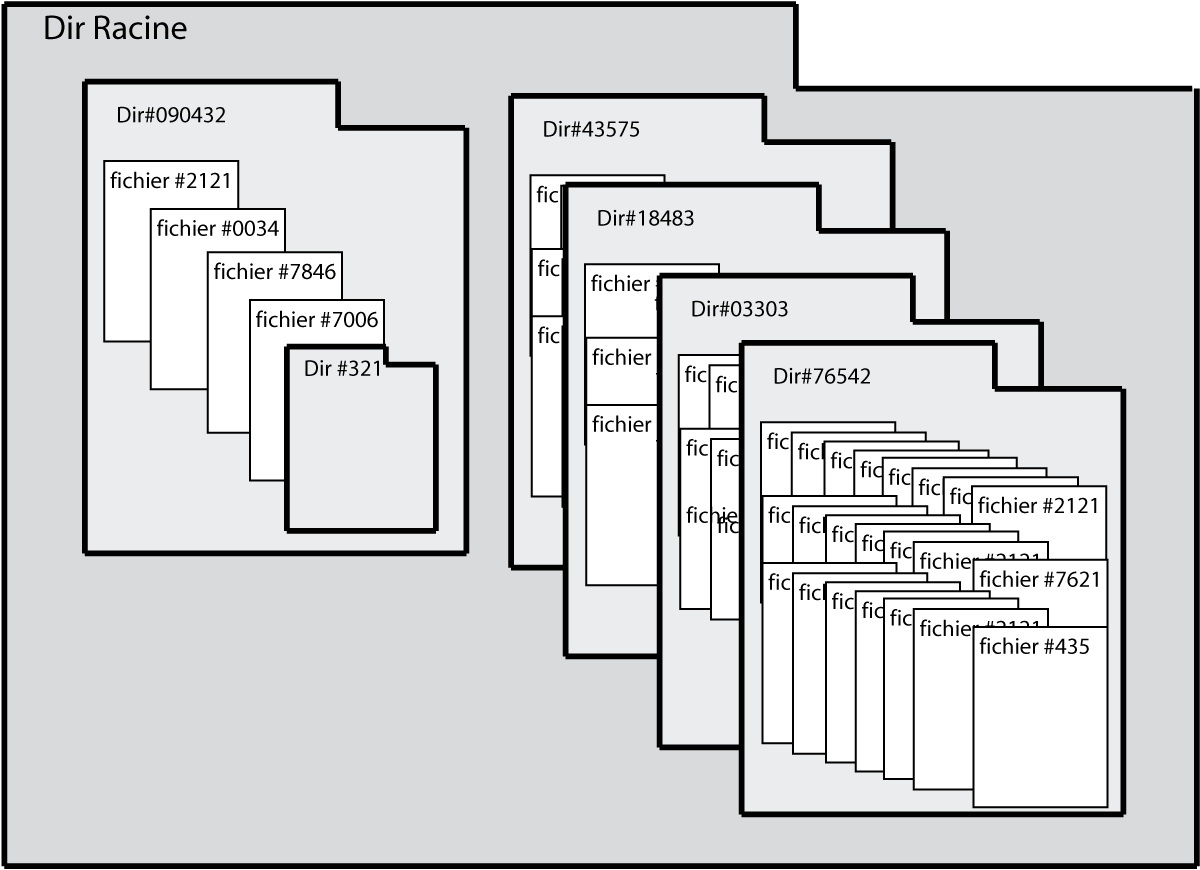
\includegraphics[width=4cm]{img/s01/file_system.jpg}
      \end{column}
    \end{columns}
  \end{block}
  \begin{block}{Une organisation en arborescence}
    \begin{itemize}
    \item Cette organisation arborescente permet de faciliter la recherche d'un fichier,
    \item Les fichiers sont regroupés par application, par thème, par format, par fonction, \dots			\end{itemize}
  \end{block}
  \begin{alertblock}{Remarque}
    \begin{itemize}
    \item Si tous les fichiers étaient au même \textit{"endroit"}, il serait très difficile de les afficher dans un navigateur. Leur affichage n'apporterait rien car il y en aurait trop à lire.
    \item L'organisation en arborescence est une organisation hiérarchique, qui permet d'organiser les données et de faciliter leur accès.
    \end{itemize}
  \end{alertblock}
\end{frame}		






